\chapter{Desarrollo}
\section{Integración de prácticas de la cultura DevOPS}
\subsection{Integración continua y despliegue continuo en el SMR}

Cada repositorio del Sistema NMS tiene dos ramas principales de git, Master y QA, la función de cada una es la siguiente:

\begin {itemize}
\item QA: esta es la rama principal para integrar todos los cambios en el código. Todo el código nuevo se prueba y analiza antes de poder enviarlo a esta rama.
\item Master: La rama de producción, donde el producto de software completa su último paso donde estará disponible para los consumidores.
\end {itemize}

\begin{figure}[H]
	\centering
	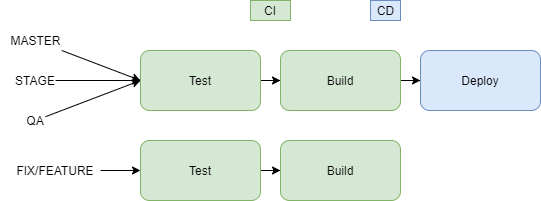
\includegraphics[width=\linewidth]{bibliografia/Imagenes/ci_cd branch Diagram.png}
	\caption{Diagrama de ramas y canales, el color indica que paso hace parte de la integración y el despliegue}
	\label{pipelines}
\end{figure}

Cada rama cuenta con  una serie de pasos como pueden observarse en la Figura \ref{pipelines} cuya función es la siguiente:
\begin{itemize}
\item Test: La aplicación de pruebas unitarias sobre todo el código para verificar la integridad del desarrollo y evitar que una funcionalidad pueda verse comprometida.
\item Build: El componente está preparado para ser implementado (crear una imagen, comprimir el código, construir el código, etc.).
\item Deploy: Despliega el componente en el entorno de desarrollo.
\end{itemize}

Como se ilustra en la Fig. \ref{pipelines}, las ramas principales (Master y QA) tienen un canal que incluye el despliegue, mientras que las ramas secundarias (con prefijo FIX/FEATURES) unicamente ejecutan los pasos de prueba y compilación, esto se debe en principio a que estas ramas son temporales y no tienen un ambiente de despliegue. Para cualquier integración es necesario que cualquier rama ejecute las pruebas unitarias y la compilación (en el caso de las ramas principales incluso el despliegue), de esta forma se verifica la integridad del código y se reduce el riesgo de llevar errores a ambientes superiores.


\subsection {Automatización de canales de los servicios del SMR}

\subsubsection {Servicios de inferencia}

En las Figuras \ref {pipelineA} y la Fig. \ref{pipelineB} se muestra el canal de los servicios de inferencia \cite{EstebanInferencerAdapa2020}, los trabajos se clasifican por etapa de la siguiente manera.

\begin {itemize}
	\item Test: Ejecuta pruebas unitarias y la verificación sonar de forma simultanea. Ambos pasos son requeridos para el build.
	\item Build: Compila y sube una imagen a AWS ECR.
	\item Deploy: Ejecuta un trabajo en un contenedor de terraform. Proporciona la infraestructura para los servicios de inferencia.
\end {itemize}

\begin{figure}[H]
\centering
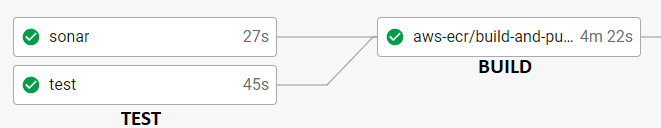
\includegraphics[width=0.8\linewidth]{bibliografia/Imagenes/inferencerpipelineA.PNG}
\caption {Parte A de la canalización del servicio de inferencia. Etapa de prueba y compilación}
\label {pipelineA}
\end {figure}

\begin{figure}[H]
\centering
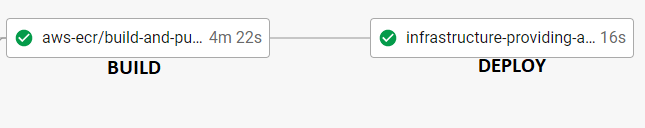
\includegraphics[width=0.8\linewidth]{bibliografia/Imagenes/inferencerpipelineB.PNG}
\caption {Canalización del servicio de inferencia, parte B, etapa de compilación e implementación}
\label {pipelineB}
\end {figure}


\subsubsection {Lambda para la publicación a Kafka}


En la Figura \ref{pipelineLambdaProducer} se muestra el canal para la Lambda de notificación a Kafka \cite{EstebanEventProducer2021}, los trabajos se clasifican por etapa de la siguiente manera.

\begin {itemize}
\item Build: Instala dependencias y genera un archivo ''zip´´ junto con el código que se almacena en el flujo de trabajo.
\item Deploy: Ejecuta un trabajo en un contenedor de terraform. Recupera ''zip´´ almacenado y lo despliega en AWS Lambda, adicionalmente crea el disparador desde S3.
\end {itemize}

\begin{figure}[H]
	\centering
	
\includegraphics[width=1\linewidth]{bibliografia/Imagenes/lambdaProducerPipeline.PNG}
	\caption {Canalización del servicio lambda}
	\label {pipelineLambdaProducer}
\end {figure}


\subsubsection {Servicio de Logstash}

En la Figura \ref{pipelineKafkaLogstash} se ilustra el canal para el servicio de logstash \ref{EstebanLogstash2021}, los trabajos se clasifican por etapa de la siguiente manera.

\begin {itemize}
\item Build: Se prepara la imagen para subirse a AWS ECR.
\item Deploy: Ejecuta un trabajo en un contenedor de terraform. Proporciona la infraestructura para el servicio de logstash.
\end {itemize}

\begin{figure}[H]
	\centering
	
\includegraphics[width=1\linewidth]{bibliografia/Imagenes/kafkaLogstashPipeline.png}
	\caption {Canalización del servicio Logstash}
	\label {pipelineKafkaLogstash}
\end {figure}
	
\subsubsection {Reutilización de variables de entorno con contextos}

Durante los despliegues (Por medio de orb o terraform), se utilizan las mismas variables de entorno por lo que no hay necesidad de repetirlas en cada proyecto, por el contrario se definen contextos.

\begin{itemize}
	\item TerraformContext: Utilizado para todos los canales que utilicen terraform para su despliegue. Se definen todas las llaves de AWS. 
	\item IACTerraformInferencer: Utilizado en todos los proyectos de los servicios de inferencia, donde se definen variables de la definición de tarea y variables de Kafka. 
\end{itemize}

En la \ref{circlecontext} se ilustra la definición de contextos para el flujo de trabajo del servicio de infererencia ADAPA, en la cual como puede observarse se definen más de un contexto

\begin{figure}[H]
	\centering
	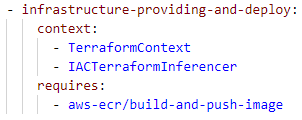
\includegraphics[width=0.7\linewidth]{bibliografia/Imagenes/contextos.png}
	\caption {Definición de contextos}
	\label {circlecontext}
\end {figure}

\subsection{IAC con Terraform}

\subsubsection{Configuración del proveedor y backend}

Los proveedores son ``plugins que implementan tipos de recursos'' \cite{terraform}, permiten el uso de terraform con un proveedor en la nube. En el SMR se utiliza el plugin de AWS.

\begin{figure}[H]
	\centering
	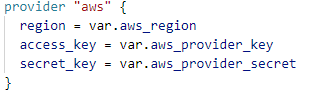
\includegraphics[width=0.7\textwidth]{bibliografia/Imagenes/providertf.PNG}
	\caption{AWS como proveedor en terraform}
	\label{providertf}
\end{figure}

Terraform mantiene un archivo de estado para mapear recursos a la configuración de terraform, seguimiento de metadatos y la mejora en el rendimiento en grandes infraestructuras \cite{terraform}. En el SMR cada servicio mantiene un archivo de estado almacenado en un bucket de S3, por lo que siempre esta disponible si se desea desplegar desde diferentes entornos de ejecución. la Figura \ref{backendtf}  muestra la configuración del backend para el servicio de inferencia (todos los servicios de SMR usan una configuración similar).

\begin{figure}[H]
	\centering
	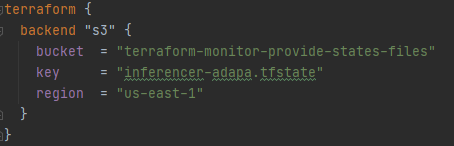
\includegraphics[width=0.8\textwidth]{bibliografia/Imagenes/backendtf.PNG}
	\caption{Definición del backend en terraform}
	\label{backendtf}
\end{figure}



\subsection{Despliegue de servicios de SMR con terraform}


La configuración detrás de cada componente del SMR involucra múltiples entidades o servicios de Amazon. La configuración de cada despliegue a mano reduce la eficiencia y puede llevar a errores o despliegues incompletos. En la Figura \ref{archcomponents} se mencionan los servicios utilizados y su relación.

\begin{figure}[H]
	\centering
	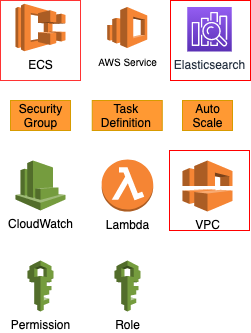
\includegraphics[width=0.80\textwidth]{bibliografia/Imagenes/Architecture Components.png}
	\caption{Componentes de AWS en el SMR}
	\label{archcomponents}
\end{figure}

Con terraform cada entidad en la figura \ref{archcomponents} es configurada una vez, luego su creación y despliegue es automático. Los componentes marcados con un recuadro rojo se llaman ``componentes compartidos'', lo que significa que son componentes a los que otras entidades están asociados, por este motivo tienen una configuración y un despliegue independiente.

\begin{figure}[H]
	\centering
	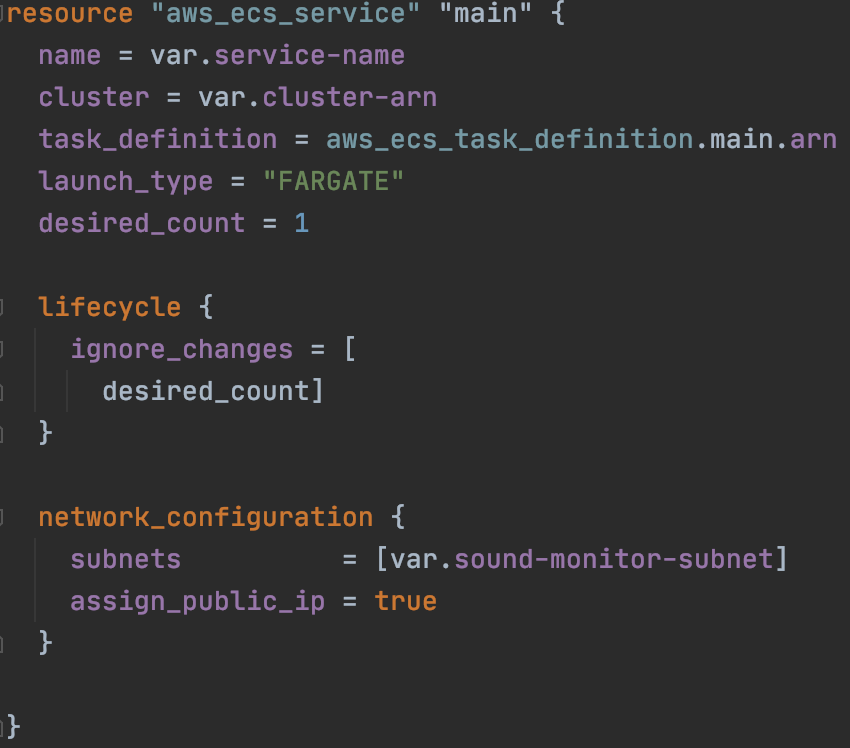
\includegraphics[width=0.8\textwidth]{bibliografia/Imagenes/infrastructure-providing.png}
	\caption{Configuración de un servicio de ECS para los servicios de inferencia}
	\label{ecsprovide}
\end{figure}

La figura \ref{ecsprovide} muestra la definición de un servicio utilizando terraform. Si algo es modificado en la configuración, terraform actualiza las entidades involucradas, sin crearlas nuevamente. En circleCI se puede monitorear el estado del despliegue de un servicio accediendo al trabajo de terraform como se muestra en la figura \ref{circleCITerraform}.

\begin{figure}[H]
	\centering
	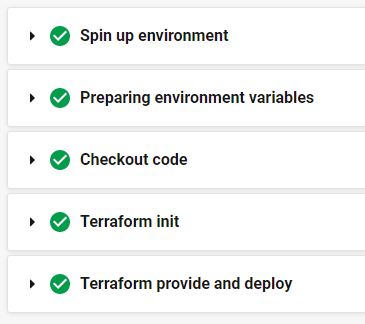
\includegraphics[width=0.7\textwidth]{bibliografia/Imagenes/circleCITerraformJob.png}
	\caption{Monitoreo de despliegue de terraform con circleCI}
	\label{circleCITerraform}
\end{figure}

\subsubsection{Usando módulos para la definición de infraestructura común}

En el SMR los servicios de inferencia (ADAPA \cite{EstebanInferencerAdapa2020} y YAMNET \cite{EstebanYAMNET2021}) cuentan con la misma infraestructura por lo que no es necesario definirla en cada repositorio (lo cual lleva a la repetición de código). Para ello se utilizan módulos cuya fuente se encuentra en un repositorio \cite{EstebanInferencerCommon2021} en donde están definidas todas las entidades utilizadas por estos servicios.

\begin{figure}[H]
	\centering
	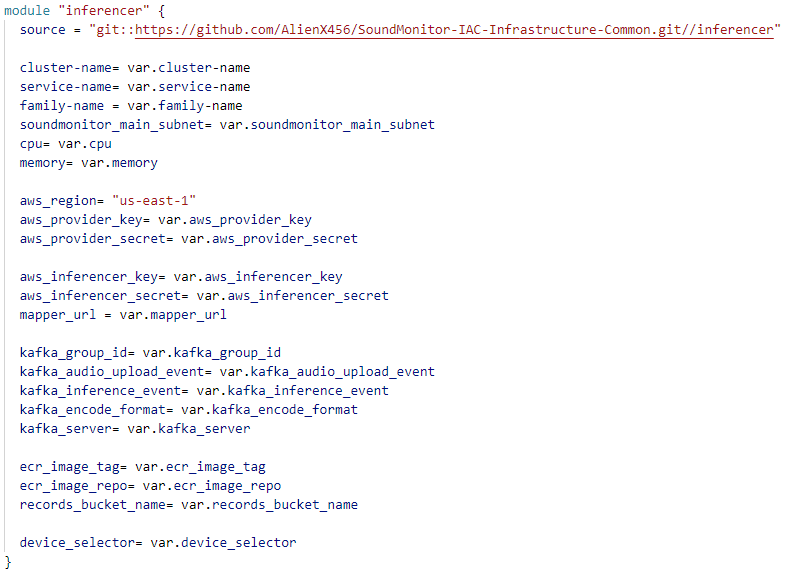
\includegraphics[width=0.8\textwidth]{bibliografia/Imagenes/moduleInferencer.png}
	\caption{Modulo para servicios de inferencia}
	\label{moduleTerraform}
\end{figure}

En la figura \ref{moduleTerraform} se define un modulo en el servicio de inferencia de ADAPA el cual recupera las entidades del repositorio definido en el atributo ``source''.

\subsection{Integración con SonarCloud}